\section{Trivial Carrier Sensing}
\label{sec:trivial}

Trivial Carrier Sensing extends the Aloha protocol described in \cref{sec:aloha} to include a carrier sensing function that tries to avoid collisions between packets.
Before sending a packet, the station listens the energy on the channel to detect possible incoming packets.
If the channel is free, the packet is transmitted immediately.
If the channel is occupied, the transmission is delayed to when the channel becomes free.

The simulator assumes that a station can correctly determine if the channel is free or not with a probability of $1$.
The station can either sense the channel, transmit, receive or process a packet at a time.
It is not possible, for instance, to sense the channel when transmitting a packet.
We assume that the station can sense the channel instantly.

Carrier sensing is introduced on end\_proc events: if the channel is not free, the node move to the new state \textbf{WC} (WAITING\_FREE\_CHANNEL) and waits until the channel is free.
When the channel gets free (end\_rx with recv\_count = 0), it moves to TX and transmit the next packet if any, otherwise to IDLE.
As a side effect, it is not possible anymore to get the events for start and end receiving in the IDLE state, since they are captured from the WC state.
\cref{fig:trivial_cs_states} shows the state machine diagram for the Trivial Carrier Sensing protocol.

\begin{figure}[h]
	\centering
	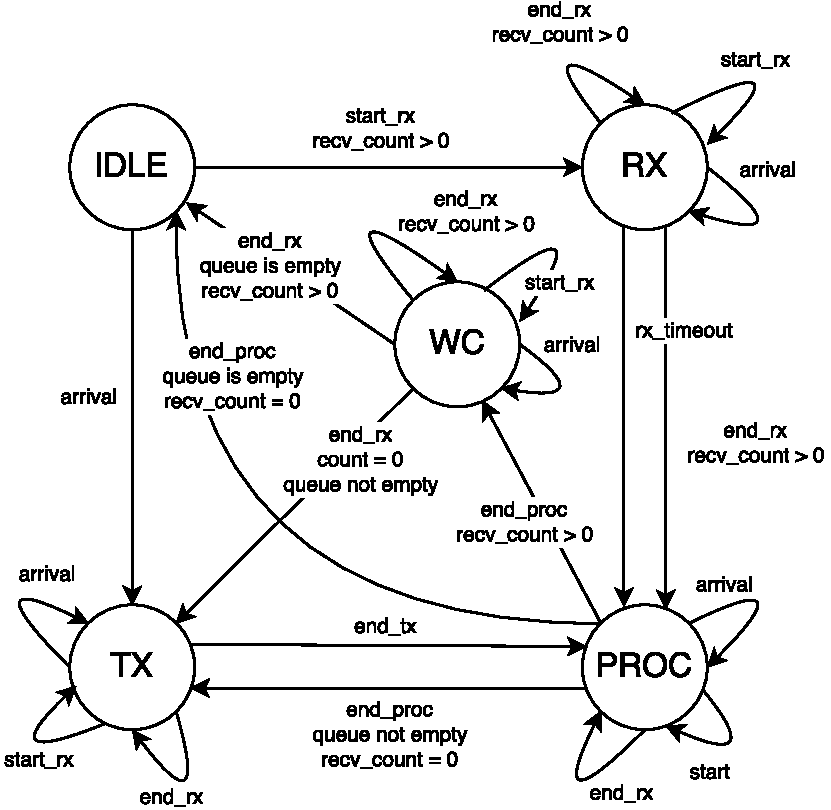
\includegraphics[width=0.95\columnwidth]{figures/states/trivial}
	\caption{State machine for a single station for Trivial Carrier Sensing.}
	\label{fig:trivial_cs_states}
\end{figure}
